A more thorough visual evaluation of nuclei fluroescence predictions is provided in Figure \ref{fig:nuclei-troubles}. There are tree main visible problems that should be adressed in further research:
\begin{itemize}
	\item The form of the nucleus is well-captured, but the texture inside is not (the change of intensities) is not predicted very well.
	\item The border around the nucleus is quite blurry
	\item The overall intensities of predictions seem to be higher than the ground truth ones.
\end{itemize}

All of these problems are quite similar and can be summarized under the statement that the model does not have enough of resolution. Which can be solved by making a model larger and providing more data to it. In order to confirm this a bigger model has been trained. 

Indeed, increasing the number of filters in each convolutional layer by a factor of $4$ (switching from from $16$ to $64$ in the first one) the model was able to capture more details. Predictions became better both visually (see Figure \ref{fig:better-nuclei}) and based on both metrics (PCC and MSE losses, see Figure \ref{fig:nuclei-comparison-predictions}).

\begin{figure}[H]
	\begin{center}
		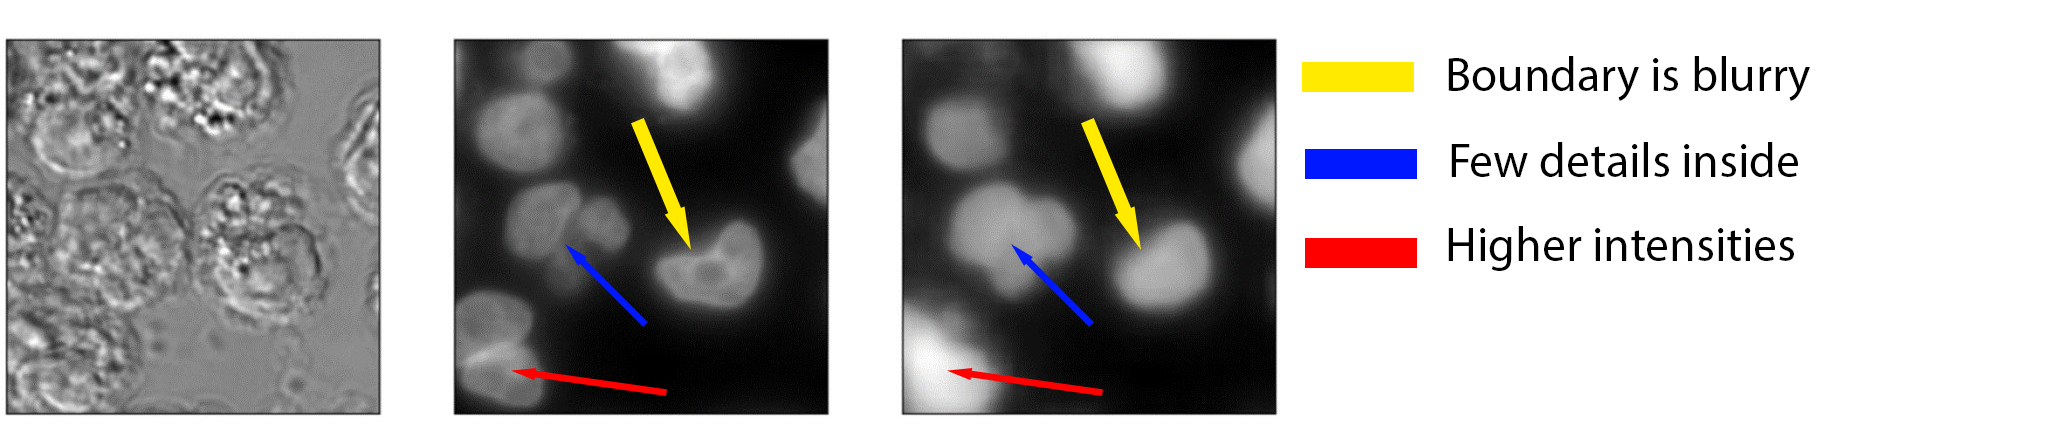
\includegraphics[width=0.8\linewidth]{bilder/nuclei/problems.png}
		\caption{Problems in predictions}\label{fig:nuclei-troubles}
	\end{center}
\end{figure}

Another rather small issue is that predictions on the border of the crops seem to be worse than in the middle. As has already been mentioned in section \ref{par:crops-combination}, when the cell is not fully present in the crop (split in halves for ex.), the network doesn't have enough data to give out a good enough prediction. However, when combining crops into a high-resolution images, this problem can be mitigated by the method described in section \ref{par:crops-combination}.

The problem of the higher intensities can also be addressed by a more careful dataset filtration, as few several images with overexposed cells are still used for training and that might be a reason of intensity overprediction. Blurry borders is also a signal of an overexposed nucleus. Even if they are present in the dataset, they can be removed using background removal techniques described in section \ref{par:background-removal}. This was not done in the scope of this research as the predictions have had good enough qulity to be used in CLD process.

\begin{figure}[H]
	\begin{center}
		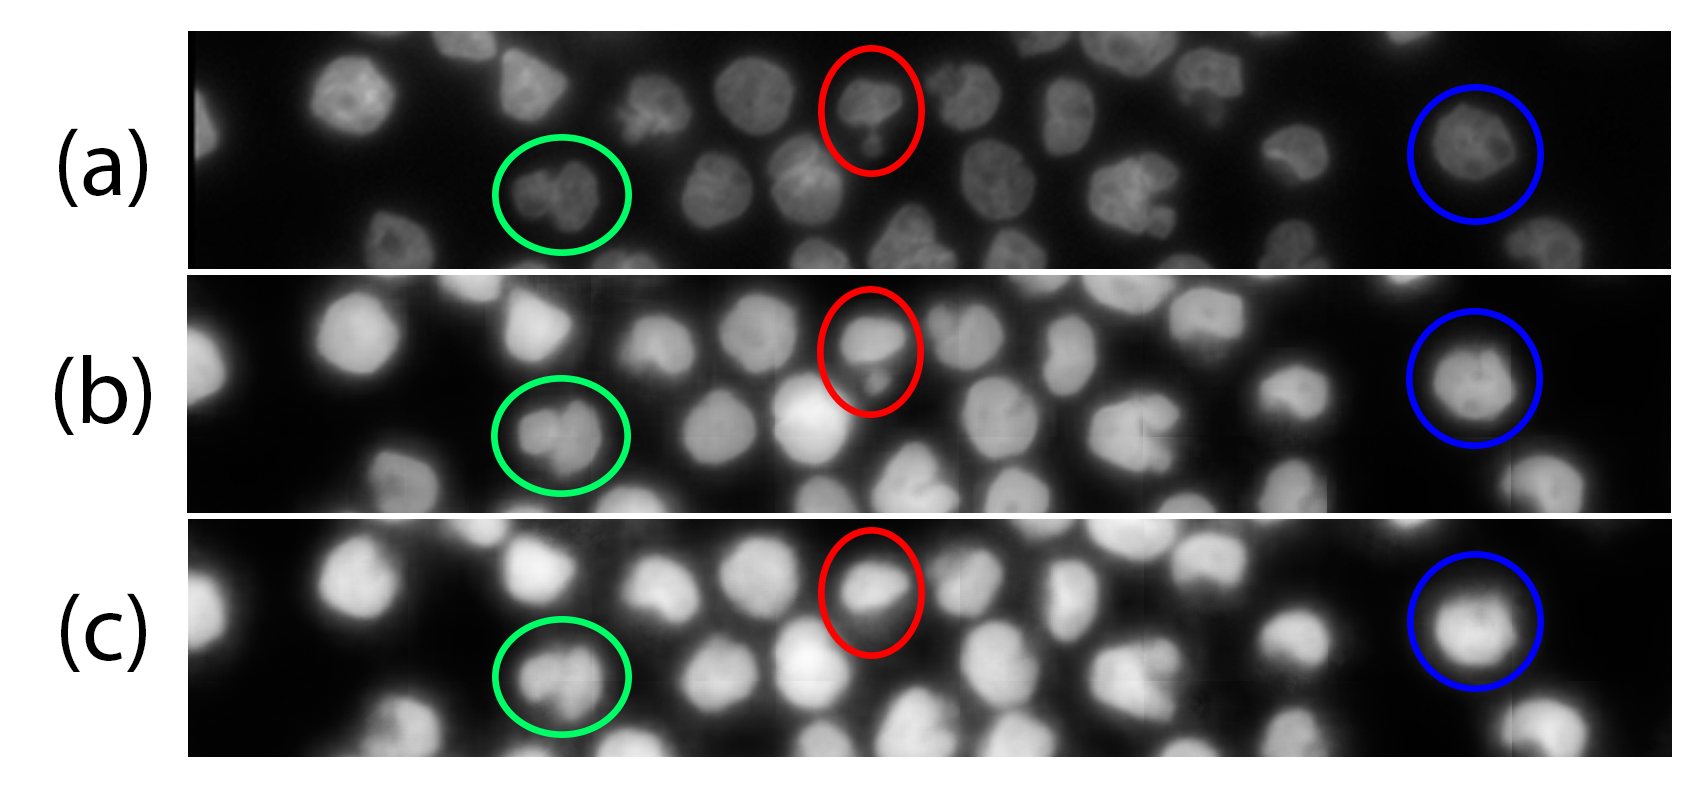
\includegraphics[width=0.6\linewidth]{bilder/nuclei/bigger-model.png}
		\caption{Predictions improvement: (a) ground truth fluorescence; (b) bigger model with four times more filters in convolutional layers; (c) standard architecture}\label{fig:better-nuclei}
	\end{center}
\end{figure}